Ve snaze \textbf{popsat jakýkoliv algoritmus} si vymysleli matematici Turingovy a RAM stroje. Jde o dva různé přístupy (modely) univerzálních počítačů/programovacích jazyků. Jinými slovy těmito stroji lze \textbf{definovat} a \textbf{provést} \textbf{libovolný algoritmus}.

Historicky prvním ,,univerzálním programovacím jazykem'' byl Turingův stroj. Byl popsán dříve, ještě před rozmachem počítačů, proto se od reálného počítače (programování) podstatně liší, na rozdíl od RAM stroje. Turingův stroj například pracuje s \textbf{celou abecedou} zatímco RAM (podobně jako počítač) s \textbf{čísly}.

\subsection{Turingův stroj (TS)}
\begin{figure}[H]
	\centering
	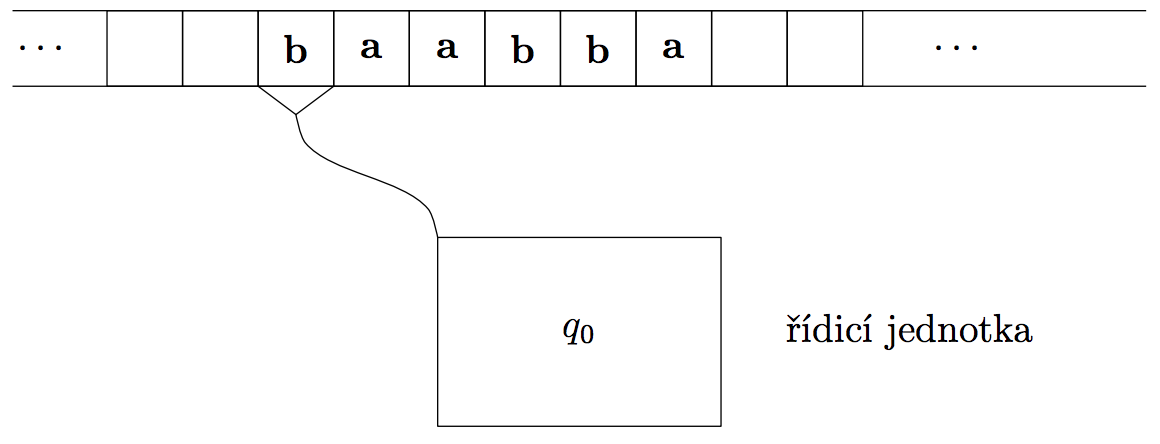
\includegraphics[width=0.8\textwidth]{assets/turing}
\end{figure}
Turingův stroj je podobný konečnému automatu, ale má \textbf{oboustranně nekonečnou pásku} (je na ni zapsáno vstupní slovo), místo symbolu $\epsilon$ pro prázdné znaky se používá $\Box$, \textbf{hlava} je \textbf{čtecí} i \textbf{zapisovací} a pohybuje se po pásce v \textbf{obou směrech}.

\subsubsection{Formální definice TS}
Turingův stroj, je definován jako šestice $M = (Q, \Sigma, \Gamma, \delta, q_0, F)$, kde:
\begin{itemize}
\item $Q$ je konečná neprázdná množina \textbf{stavů}.
\item $\Sigma$ je konečná neprázdná množina \textbf{vstupních symbolů} (vstupní abeceda).
\item $\Gamma$ je konečná neprázdná množina \textbf{páskových symbolů}, kde $\Sigma \subseteq \Gamma$ a $\Gamma - \Sigma$ je (přinejmenším) speciální znak $\Box$ (prázdný znak [Blank]).
\item $\delta$ je přechodová funkce, $\delta: (Q - F) \times \Gamma \rightarrow Q \times \Gamma \times \{-1, 0, +1\}$.
\item $q_0$ je \textbf{počáteční stav}, $q_0 \in Q$.
\item $F$ je množina \textbf{koncových stavů}, $F \subseteq Q$.
\end{itemize}

\subsubsection{Definice instrukcí (pravidel) v TS}
Podobně jako ZA lze konkrétní Turingův stroj zadat seznamem instrukcí. Tyto instrukce jsou opět dány přechodovou
funkcí, význam instrukce: $(q, a) \rightarrow (q', a', m)$ je tento:
\begin{center}
(akt. stav [$q$], znak na pásce [$a$]) $\rightarrow$ (\textbf{nový stav} [$q'$], \textbf{nový znak} [$a'$], \textbf{posun} [$\{-1;0;+1\}$])
\end{center}
\subsubsection{Příklad}
Tento příklad invertuje slovo, které je uvedené na úvodním obrázku u TS:
\begin{center}
\begin{minipage}[t]{0.3\textwidth}
$Q = \{q_1, q_2\}$\\
$\Sigma = \{a, b, c, \Box\}$\\
$q_0 = q_1$\\
$F = \{q_2\}$\\
\end{minipage}
\begin{minipage}[t]{0.3\textwidth}
$(q_1, a) \rightarrow (q_1, b, +)$\\
$(q_1, b) \rightarrow (q_1, a, +)$\\
$(q_1, \Box) \rightarrow (q_2, \Box, 0)$
\end{minipage}
\end{center}

\subsubsection{Modifikace TS}
\begin{itemize}
\item \textbf{N-páskový TS} -- \textbf{čte} a \textbf{zapisuje} do \textbf{více pásek} najednou, jediná změna je v přechodové funkci: $\delta :Q\times \Gamma ^{n}\rightarrow Q\times (\Gamma \times \{L,R,N\})^{n}$.
\item \textbf{N-hlavový TS} -- má více čtecích hlav než klasický TS, každá hlava zapisuje/čte a pohybuje se \textbf{nezávisle na ostatních}.
\item \textbf{Nedeterministický TS} -- umožňuje výběr z více možností, pro jednu konfiguraci můžeme definovat \textbf{více pravidel}.
\end{itemize}

\subsubsection{Základní pojmy}
\begin{itemize}
\item \textbf{Turingovsky úplný} -- stroj (počítač, programovací jazyk, úloha, ...), která má stejnou výpočetní sílu jako TS. Lze v něm \textbf{odsimulovat} libovolný jiný TS zadaný na vstupu.
\item \textbf{Church-Turingova teze} -- říká, že jakýkoliv výpočet lze úspěšně uskutečnit algoritmem běžícím na počítači, tedy ,,ke každému algoritmu existuje ekvivalentní TS''.
\end{itemize}

\subsection{Model RAM (Random Access Machine)}
RAM stroje již vycházejí ze skutečných počítačů, dá se tedy říct, že se jedná o jednoduchou abstrakci reálného procesoru s jeho strojovým kódem pracujícím s lineárně uspořádanou pamětí. Tento model slouží zejména k analýzy algoritmů z hlediska (\textbf{paměťové}, \textbf{časové}) \textbf{složitosti}. Skládá se z těchto částí:
\begin{enumerate}
\item \textbf{Programová jednotka} -- uchovává program, tvořený konečnou posloupností instrukcí.
\item \textbf{Neomezená pracovní paměť} -- neomezená lineárně uspořádaná paměť, tvořená buňkami, do který lze zapisovat/číst celá čísla ($\mathbb{Z}$), adresovaná přirozenými čísly ($\mathbb{N}$) (0 = \textbf{pracovní} registr, 1 = \textbf{indexový} registr).
\item \textbf{Vstupní a výstupní páska} -- lze na ně sekvenčně zapisovat/číst celá čísla ($\mathbb{Z}$).
\item \textbf{Centrální jednotka} -- obsahuje programový register ukazující, která instrukce má být provedena. Ta se provede a programý registr se příslužně změní (zvýší o 1, o více v případě skoku).
\end{enumerate}

\begin{figure}[!ht]
\centering
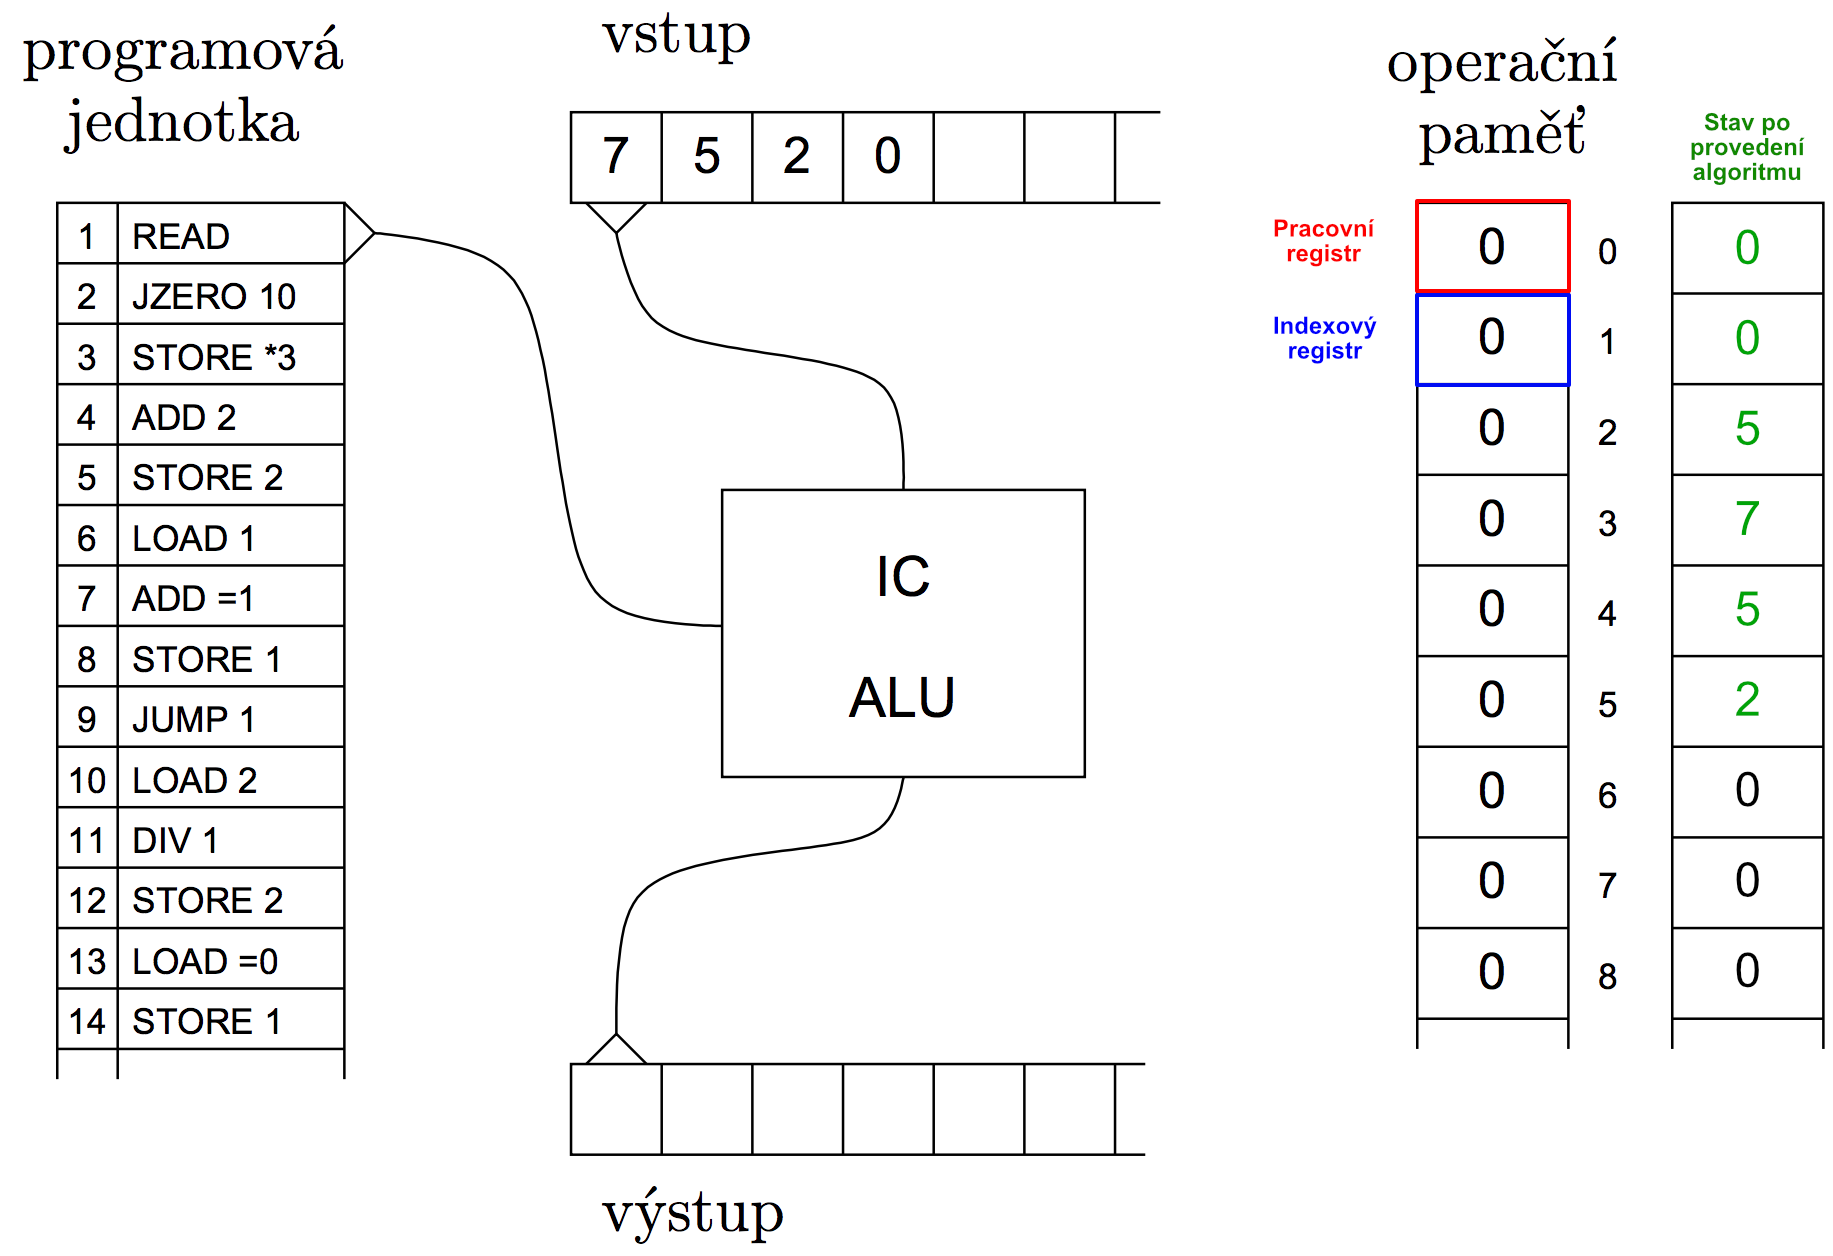
\includegraphics[width=0.63\textwidth]{assets/ram}
\end{figure}

Výše uvedený program vypočítá \textbf{aritmetický průměr}, který následně uloží do buňky paměti pod indexem č. \textbf{2}. Výsledek po dělení je roven $4,666$ a po zaokrouhlení $5$.

\subsubsection{Instrukce a typy operandů RAM}
\begin{table}[H]
\centering
\begin{tabular}{l|l}
\textbf{Typ} & \textbf{Hodnota operandu} \\ \hhline	
$=i$ & přímo číslo udané zápisem $i$  \\
$i$ & číslo obsažené v buňce s adresou $i$   \\
$*i$ & číslo v buňce s adresou $i + j$, kde $j$ je aktuální obsah indexového registru
\end{tabular}
\end{table}

\begin{table}[H]
\centering
\begin{tabular}{l|l}
\textbf{Zápis} & \textbf{Význam} \\ \hhline	
\texttt{READ} & do pracovního registru (PR) se \textbf{načte} vstup a hlava se posune
doprava \\
\texttt{WRITE} & na výstup se \textbf{zapíše} hodnota PR \\
\texttt{LOAD} $op$ & do PR se \textbf{načte} hodnota dána operátorem $op$  \\
\texttt{STORE} $op$ & hodnota PR se \textbf{uloží} na do registru daného operátorem $op$ \\
\texttt{ADD} $op$ & k hodnotě PR se \textbf{přičte} hodnota daná operátorem $op$  \\
\texttt{SUB} $op$ &  od hodnoty v PR se \textbf{odečte} hodnota daná operátorem $op$ \\
\texttt{MUL} $op$ &  PR se \textbf{vynásobí} hodnotou danou operátorem $op$ \\
\texttt{DIV} $op$ &  PR se \textbf{vydělí} hodnotou danou operátorem $op$ \\
\texttt{JUMP} \textit{návěští} & provede se \textbf{skok} na instrukci danou \textit{návěštím} \\
\texttt{JZERO} \textit{návěští} & pokud je hodnota v \textbf{PR rovna 0}, provede se skok na \textit{návěští} \\
\texttt{JGTZ} \textit{návěští} & pokud je hodnota v \textbf{PR větší než 0}, provede se skok na \textit{návěští} \\
\texttt{HALT} & \textbf{korektní ukončení} programu \\

\end{tabular}
\end{table}

\subsection{Složitost algoritmů}
Abychom mohli \textbf{porovnávat} různé algoritmy řešící stejný problém, zavádí se pojem složitost algoritmu. Složitost je jinak řečeno \textbf{náročnost algoritmu} -- čím menší složitost tím je algoritmus lepší.
Přičemž nás může zajímat složitost z pohledu \textbf{času}, či \textbf{paměti}:
\begin{itemize}
\item \textbf{Časová složitost} -- sleduje jak závisí \textbf{doba} výpočtu alg. na množství vstupních dat.
\item \textbf{Prostorová složitost} -- sleduje jak závisí \textbf{množství použité paměti} výpočtu alg. na množství vstupních dat.
\end{itemize}
Jelikož konkrétní čísla (čas, bity) se liší v \textbf{závislosti vstupních datech}, množství zpracovávaných dat a použitém programovacím jazyku, neudává se složitost čísly, nýbrž \textbf{funkcí závislou na velikosti vstupních dat}. Tato funkce se získá počítáním proběhlých instrukcí algoritmu sestaveném v univerzálním RAM stroji. A počítá se s nejhorším možným případem vstupu. To je důležité například u třídících algoritmů, kde hraje velkou roli to, jak moc už je vstupní pole setříděné (vstupuje-li do algoritmu už setříděná posloupnost čísel, algoritmus skončí okamžitě, zatímco s opačně seřazenými čísly se bude trápit dlouho.

\subsection{Asymptotická notace}
Je \textbf{způsob klasifikace počítačových algoritmů}. Ve většině případů nemusíme znát přesný počet provedených instrukcí a spokojíme se pouze s odhadem toho, jak rychle tento počet narůstá se zvyšujícím se vstupem. Asymptotická notace nám umožní \textbf{zanedbat méně důležité detaily} a \textbf{odhadnout} přibližně, \textbf{jak rychle daná funkce roste}.
 V souvislosti s asymptotickými odhady složitosti se používjí tyto zapisy:
\begin{itemize}
	\item $f \in O(f)$ -- $f$ roste \textbf{nejvýše tak rychle} jako $g$ ($f$ je ohraničena $g$ \textbf{shora}) $[\leq]$.
	\item $f \in o(g)$ -- $f$ roste \textbf{(striktně) pomaleji} než $g$ ($f$ je ohraničena $g$ \textbf{shora ostře}) $[<]$.
	\item $f \in \Theta (g)$ -- $f$ roste \textbf{stejně rychle} jako $g$ $[=]$.
	\item $f \in \omega(g)$ -- $f$ roste \textbf{(striktně) rychleji} než $g$ ($f$ je ohraničena $g$ \textbf{zdola ostře}) $[>]$.
	\item $f \in \Omega(g)$ -- $f$ roste \textbf{rychleji} než $g$ ($f$ je ohraničena $g$ \textbf{zdola}) $[\geq]$.
\end{itemize}

\begin{minipage}{0.4\textwidth}
\begin{figure}[H]
	\centering
	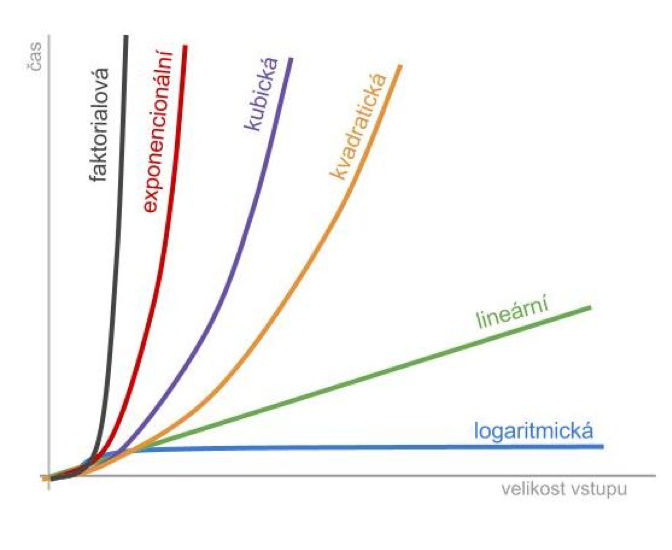
\includegraphics[width=\textwidth]{assets/asympt}
\end{figure}
\end{minipage}
\begin{minipage}{0.6\textwidth}
\textbf{Seřazeno podle složitosti}:
\small
\begin{itemize}
\item $f(n) \in \Omega(log n)$ -- logaritmická funkce (složitost),
\item $f(n) \in \Omega(n)$ -- lineární funkce (složitost),
\item $f(n) \in \Omega(n^2)$-- kvadratická funkce (složitost),
\item $f(n) \in O(n^k)$ pro nějaké $k > 0$ -- polynomiální,
\item $f(n) \in \Omega(k^n)$ pro nějaké $k > 1$ -- exponenciální.
\end{itemize}
\end{minipage}

\subsubsection{Úskalí asymptotické notace}
Při používání asymptotických odhadů časové složitosti je třeba si uvědomit některá úskalí:
\begin{itemize}
	\item Asymptotické odhady se týkají pouze toho,\textbf{ jak roste čas s rostoucí velikostí vstupu} $\rightarrow$ neříkají nic o \textbf{konkrétní době výpočtu}. V asymptotické notaci mohou být \textbf{skryty velké konstanty}.
	\item Algoritmus, který má lepší asymptotickou časovou složitost než nějaký jiný algoritmus, \textbf{může být ve skutečnosti rychlejší} až pro nějaké hodně velké vstupy.
	\item Většinou analyzujeme složitost v \textbf{nejhorším případě}. Pro některé algoritmy může být doba výpočtu v nejhorším případě mnohem větší než doba výpočtu na „typických“ instancích (typicky Quicksort $\rightarrow$ nejhorší: $O(n^2)$, průměrná: $O(n \log n)$).
\end{itemize}

\subsection{Algoritmicky nerozhodnutelné problémy}
Rozhodovací problém je rozhodnutelný (řešitelný) pokud pro libovolný vstup z množiny vstupů, skončí algoritmus svůj výpočet a vydá správný výstup (tedy jestliže \textbf{existuje turingův stroj, který jej řeší}).

Pokud nalezneme takový vstup, pro který všechny dosavadní algoritmy nejsou schopny nalézt výstup, můžeme tento problém označit za \textbf{nerozhodnutelný}. Speciální případ jsou \textbf{doplňkové problémy}, které vracejí přesně opačné výsledky než původní problém.

\subsubsection{Definice problému}
Problém je určen \textbf{trojicí} $(IN, OUT, p)$, kde:
\begin{itemize}
\item $IN$ je množina (přípustných) \textbf{vstupů},
\item $OUT$ je množina \textbf{výstupů},
\item $p: IN \rightarrow OUT$ je \textbf{funkce} přiřazující každému vstupu odpovídající výstup. 
\end{itemize}

\subsubsection{Ano/Ne problémy}
Jsou to problémy, jejichž \textbf{výstupní množina obsahuje dva prvky} $OUT=\{\rm ano, ne\}$.
 Na ano/ne problémy se dají převést ostatní problémy nepotřebujeme-li znát přesný výsledek:
\begin{itemize}
\item Nepotřebuji najít v poli nejmenší číslo, stačí mi vědět \textbf{zda pole obsahuje číslo menší než nula}.
\item Nepotřebuji znát nejkratší cestu grafem, stačí mi najít cestu, \textbf{která je kratší než 8}.
\end{itemize}

\subsubsection{Riceova věta}
Tato věta ukazuje nerozhodnutelnost celé třídy problémů, její znění je následující ,,\textit{Každá netriviální vstupně/výstupní (I/O) vlastnost programů je \textbf{nerozhodnutelná}}''.

\begin{itemize}
\item Vlastnost X \textbf{je vstupně/výstupní} právě tehdy, když každé dva programy se stejnou I/O tabulkou buď oba vlastnost X mají nebo ji oba nemají.
\item Připomeňme tedy ještě, že vlastnost V je \textbf{triviální}, když ji mají buď všechny programy nebo ji nemá žádný program; taková vlastnost je podle definice také \textbf{vstupně/výstupní}.
\end{itemize}

\begin{table}[H]
	\centering
	\begin{tabular}{l|c|c|c}
		\textbf{Problém}            & \textbf{1} & \textbf{2} & \textbf{3} \\\hhline
		\textbf{Je triviální?}      &     A       &      N      &      N      \\ 
		\textbf{Je I/O?}            &   A         &        A    &        N    \\
		\textbf{Je nerozhodnutelný} &         N   &       A     &           N
	\end{tabular}
\end{table}

\subsubsection{Částečná rozhodnutelnost}
Částečně rozhodnutelný problém, je takový problém, pro který jsme v případě vstupů, u nichž očekáváme odpověď ANO, \textbf{schopni vrátit odpověď ANO}, a v případě NE vrátit buď NE nebo $\perp$ (program se nezastaví a nejsme schopni zjistit, zda by odpověď byla opravdu NE).

\subsubsection{Převeditelnost mezi nerozhodnutelnými problémy}
Důkaz neřešitelnosti lze provést skrze jiné, \textbf{už dokázané}, problémy. Řekneme, že problém $P_1$ je převeditelný na problém $P_2$ (značíme $P_1 \rightsquigarrow P_2$), jestliže alg., který k instanci $I_1$ problému $P_1$ sestrojí instanci $I_2$ problému $P_2$ tak, \textbf{že odpověď $P_1, I_1$ je stejná jako $P_2, I_2$}. Např.: DHP je převeditelný na HP.  Z toho vyplývá, že pokud $P_1$ je nerozhodnutelný tak i $P_2$ je \textbf{nerozhodnutelný}.

\subsubsection{Optimalizační problémy}
Optimalizační problémy \textbf{hledají nejlepší řešení} v množině různých řešení. Příkladem je například: hledání nejkratší cesty, nejmenší kostry, apod.

\subsubsection{Příklady optimalizačních problémů}
\begin{enumerate}
\item \textbf{Hledání nejkratší cesty v grafu}
\begin{itemize}
	\item \textbf{\textsc{Vstup}}: Orientovaný graf $G = (V, E)$ a dvojice vrcholů $u, v \in V$.
	\item \textbf{\textsc{Výstup}}: Nejkratší cesta z $u$ do $v$.
\end{itemize}
\item \textbf{Hledání minimální kostry v grafu}
\begin{itemize}
\item \textbf{\textsc{Vstup}}: Neorientovaný souvislý graf $G = (V_G,E_G)$ s ohodnocenými hranami. 
\item \textbf{\textsc{Výstup}}: Souvislý graf $H = (V_H,E_H)$, kde $V_H = V_G$ a $E_H \subseteq E_G$, který má součet hodnot všech hran minimální.
\end{itemize}
\item \textbf{Eq-CFG (Ekvivalence bezkontextových gramatik)}
\begin{itemize}
\item \textbf{\textsc{Vstup}}: Dvě bezkontextové gramatiky $G1, G2$.
\item \textbf{\textsc{Otázka}}: Platí $L(G1) = L(G2)$? Generují obě gramatiky stejný jazyk?
\end{itemize}
\item \textbf{HP (Problém zastavení [Halting Problem])}
\begin{itemize}
\item \textbf{\textsc{Vstup}}: Turingův stroj $M$ a jeho vstup $w$.
\item \textbf{\textsc{Otázka}}: Zastaví se $M$ na $w$ (tzn. je výpočet stroje M pro vstupní slovo $w$ konečný)?
\end{itemize}
\end{enumerate}


\begin{figure}[H]
	\centering
	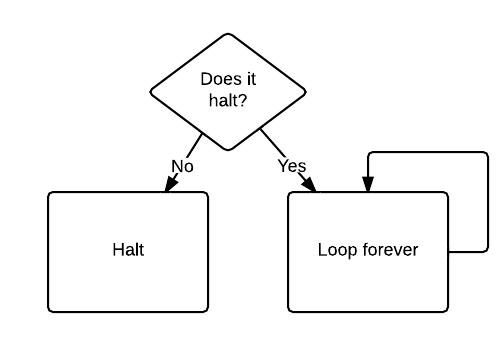
\includegraphics[width=0.5\textwidth]{assets/halting}
\end{figure}